\documentclass[10pt,twocolumn,letterpaper]{article}

\usepackage{cvpr}
\usepackage{times}
\usepackage{epsfig}
\usepackage{graphicx}
\usepackage{multirow}
\usepackage{amsmath}
\usepackage{amssymb}
\usepackage[pagebackref=true,colorlinks,linkcolor=red,citecolor=green,breaklinks=true,bookmarks=false]{hyperref}
\cvprfinalcopy
\def\cvprPaperID{****}
\def\httilde{\mbox{\tt\raisebox{-.5ex}{\symbol{126}}}}
\setcounter{page}{1}
\begin{document}
\title{SUSAN~\cite{Liu2008Shape}--A New Approach to Low Level Image Processing}
\author{Qi Zhao\\\\June 10, 2018}

\maketitle
\section{Introduction}
This paper describes a new approach to low level image processing; in particular, edge and corner detection and structure preserving noise reduction. Non-linear filtering~\cite{kallianpur1972stochastic} is used to define which parts of the image are closely related to each individual pixel; each pixel has associated with it a local image region which is of similar brightness to that pixel. The new feature detectors are based on the minimization of this local image region, and the noise reduction method uses this region as the smoothing neighborhood. The resulting methods are accurate, noise resistant and fast.
\par The SUSAN principle is now introduced, from which the research described in this paper is derived. Consider Figure~\ref{fig:onecol}, showing a dark rectangle on a white background. A circular mask (having a centre pixel which shall be known as the "nucleus") is shown at five image positions. If the brightness of each pixel within a mask is compared with the brightness of that mask's nucleus then an area of the mask can b e defined which has the same (or similar) brightness as the nucleus. This area of the mask shall b e known as the "USAN", an acronym standing for ��Univalue Segment Assimilating Nucleus~\cite{hess2004facial}". In Figure~\ref{fig:short} each mask from Figure ~\ref{fig:onecol} is depicted with its USAN shown in white. This concept of each image point having associated with it a local area of similar brightness is the basis for the SUSAN principle. The local area or USAN contains much information about the structure of the image. It is effectively region ?nding on a small scale. From the size, centroid and second moments of the USAN two dimensional features and edges can b e detected. This approach to feature detection has many differences to the well known methods, the most obvious being that no image derivatives are used and that no noise reduction is needed, which explains why the performance in the presence of noise is good.

\begin{figure}[h]
\begin{center}
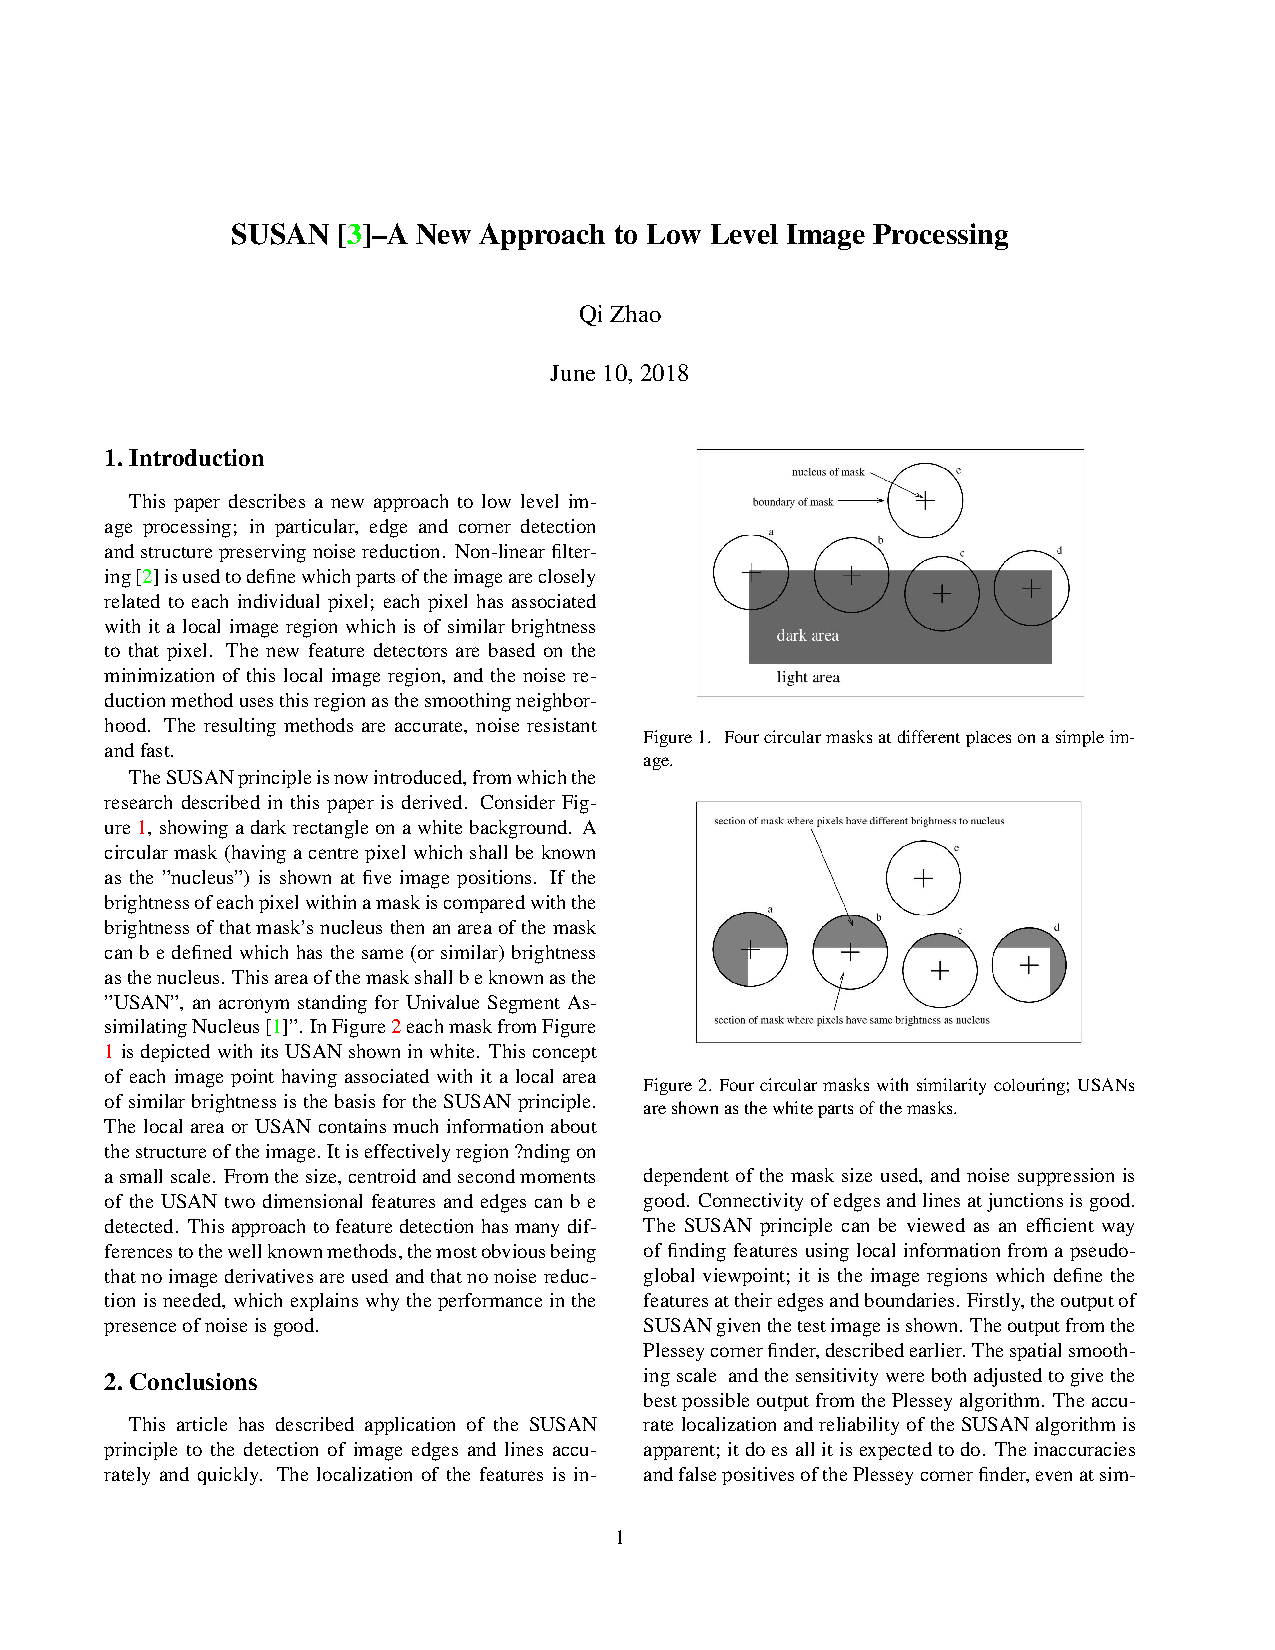
\includegraphics[width=0.8\linewidth]{SUSAN.JPG}
\end{center}
 \caption{ Four circular masks at different places on a simple image.}
\label{fig:long}
\label{fig:onecol}
\end{figure}
\begin{figure}[h]
\begin{center}
\includegraphics[width=0.8\linewidth]{SUSAN1.JPG}
\end{center}
 \caption{Four circular masks with similarity colouring; USANs are shown as the white parts of the masks.}
\label{fig:long}
\label{fig:short}
\end{figure}
\section{Conclusions}
This article has described application of the SUSAN principle to the detection of image edges and lines accurately and quickly. The localization of the features is independent of the mask size used, and noise suppression is good. Connectivity of edges and lines at junctions is good. The SUSAN principle can be viewed as an efficient way of finding features using local information from a pseudo-global viewpoint; it is the image regions which define the features at their edges and boundaries. Firstly, the output of SUSAN given the test image is shown. The output from the Plessey corner finder, described earlier. The spatial smoothing scale �� and the sensitivity were both adjusted to give the best possible output from the Plessey algorithm. The accurate localization and reliability of the SUSAN algorithm is apparent; it do es all it is expected to do. The inaccuracies and false positives of the Plessey corner finder, even at simple two region corners, are visible. This is fully explained. With respect to speed, SUSAN to ok 0.3 seconds to process this picture on a single Sun SPARC-2 processor; the Plessey corner finder took 3.5 seconds. What's more,the SUSAN algorithm has also been tested with respect to its sensitivity to noise. The results are excellent; the quality of its output (both the reliability and localization) degrades far less quickly than other algorithms tested as noise in the image is increased. The test image used was the same as the noisy image previously used to test edge finders. The outputs of SUSAN and the Plessey corner finder are shown in Figures~\ref{fig:one} and ~\ref{fig:two} respectively.
\begin{figure}[t]
\begin{center}
\includegraphics[width=0.7\linewidth]{SUSAN2.JPG}
\end{center}
 \caption{ Output of the SUSAN "corner" finder (t=10) given the test image with Gaussian noise of minimum SNR=5 added.}
\label{fig:long}
\label{fig:one}
\end{figure}
\begin{figure}[t]
\begin{center}
\includegraphics[width=0.7\linewidth]{SUSAN3.JPG}
\end{center}
 \caption{ Output of the Plessey "corner" finder (�� =2.0) given the test image with Gaussian noise of minimum SNR=5 added.}
\label{fig:long}
\label{fig:two}
\end{figure}

{\small
\bibliographystyle{ieee}
\bibliography{26}
}


\end{document}

